\documentclass{article}
\usepackage{graphicx} % Required for inserting images
\usepackage{CJKutf8}
\usepackage{amsthm}
\usepackage{mdframed}
\usepackage{float}

% 自定義 "Definition" 環境
\newmdtheoremenv{definition}{Definition}

\title{hw10}
\author{110201534 楊成偉}
\date{}

\begin{document}
\begin{CJK*}{UTF8}{bkai}
\maketitle

\section*{problem 1}
\textbf{False.} By definition, 
$val(f) = f^+(s) - f^-(s)$,
where \( f^+(s) \) represents the flow out of the source \( s \), and \( f^-(s) \) represents the flow into \( s \). It is possible for all the flow to be directed toward the source (e.g., if \( s \) become sink and \( t \) become source. In such cases, \( f^+(s) = 0 \), and val(f) would be negative.

\section*{problem 2}
\begin{figure}[H]
    \centering
    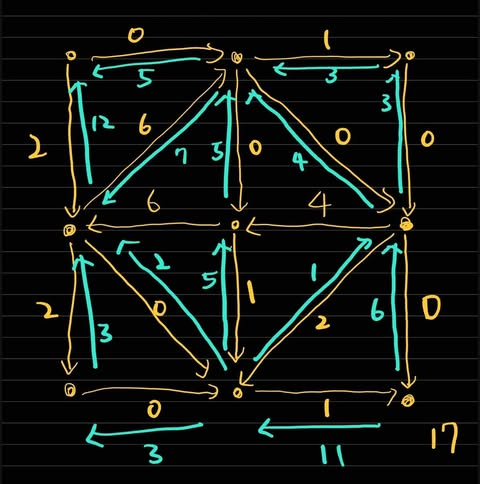
\includegraphics[scale = 0.3]{hw10.png}
    \caption{graph after ford-fulkerson algorithm}
\end{figure}

by the graph above, we can find the value of flow is 17.

\begin{figure}[H]
    \centering
    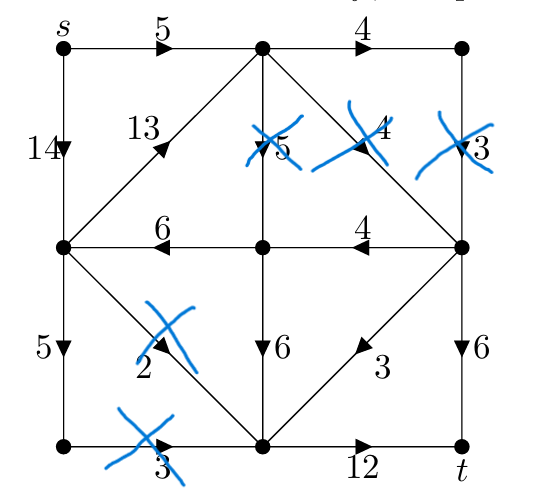
\includegraphics[scale = 0.3]{hw10cut.png}
    \caption{giving a cut that cap(S,T) is val(f)}
\end{figure}

\section*{problem 3}
\subsection*{step1}
 Construct a network N with V(N) = $\{s,t\}\cup  A \cup B$, where A = \{a1,...,ap\},B = \{b1,...,bq\}, where q means the number of groups.
 Moreover, E(N) = $\{sai : ai \in A\} \cup \{bjt : bj \in B\} \cup \{aibj : ai \in A,bj \in B\}$. Note that N is a
 digraph.
\subsection*{step2}
for each $a_{i} \in A$, let $c(sa_{i}) = m_{i}$(means every company can sent $m_{i}$ representatives) and for each $b_{j} \in B$(means every groups consist of $n_{j} participants$), let $c(b_{j}t) = n_{j}$
\subsection*{step3}
for each $a_{i} \in A, b_{j} \in B$, we let $c(a_{i}b_{j}) = 1$
\subsection*{step4}
suppose there is a representative of company i, and he is assigned to group j, we can consider this relation in the network as a flow from source to sink pass through $a_{i}, b_{j}$, since participants from the same company must be in different groups, so the capacity between $a_{i}$ and $b_{j}$ is 1.
\subsection*{step5}
if the constraints can be satisfied, means all participants can be arranged to each groups, so the max flow is $\sum_{i=1}^{p} m_{i}$
\end{CJK*}
\end{document}
